\documentclass{article}

\usepackage[slovene]{babel}
\usepackage[T1]{fontenc}
\usepackage[utf8]{inputenc}
\usepackage{listings}
\usepackage{amsmath}
\usepackage{float}
\usepackage{graphicx}
\usepackage{lmodern} 
\usepackage[a4paper, total={6in, 8in}]{geometry}

\title{Projektna naloga iz statistike}
\author{Andraž Čepič}
\date{2. 6. 2022}

\DeclareMathOperator{\std_err}{SE}

\begin{document}

\maketitle

V projektu ves čas uporabljamo Python s paketi Pandas, NumPy, Jupyter in Matplotlib.

\section*{Naloga 1}
V namen obdelave podatkov smo napisali Jupyter zvezek \texttt{kibergrad.ipynb}. Za začetek naložimo podatke iz datoteke \texttt{kibergrad.csv} v Pandas DataFrame objekt. 

\subsection*{(a)}
Izberemo enostavni slučanji vzorec velikosti $200$ s funkcijo \texttt{pandas.DataFrame.sample}. Če so
\begin{equation*}
    X_1, \ldots, X_{200}
\end{equation*}
števila otrok vsake od vzorčenih družin, je primerna ocena za povprečje enaka
\begin{equation*}
    \overline{X} = \frac{X_1 + \cdots + X_{200}}{200}.
\end{equation*}
Za naš specifičen vzorec dobimo oceno za povprečno število otrok v mestu Kibergrad:
\begin{equation*}
    \overline{X} = 0{,}925
\end{equation*}

\subsection*{(b)}
Ocena za standardno napako je podana s formulo
\begin{equation*}
    \widehat{\std_err}^2 = \frac{N-1}{N} \cdot \frac{1}{n(n-1)}\sum_{i=1}^{n}(X_i - \overline{X})^2,
\end{equation*}
kjer je $N$ velikost populacije in $n$ velikost enostavnega slučanega vzorca. V našem primeru je $N = 43.886$ in $n = 200$. Tako za naš vzorec dobimo
\begin{equation*}
    \widehat{\std_err} = 0{,}0808
\end{equation*}

Za enostavno slučajno vzorčenje so intervali zaupanja ocen povprečja oblike
\begin{equation*}
    \overline{X} - \widehat{\std_err} \cdot F^{-1}_{t}(1 - \frac{\alpha}{2}) < \mu < \overline{X} + \widehat{\std_err} \cdot F^{-1}_{t}(1 - \frac{\alpha}{2}),
\end{equation*}
kjer je $F_t$ komulativna funkcija Studentove $t$-porazdelitve z $n-1$ prostostnimi stopnjami in $\alpha = 0.05$ stopnja tveganja. V našem primeru dobimo interval zaupanja
\begin{equation*}
    0{,}7657 < \mu < 1{,}0843
\end{equation*}

\subsection*{(c)}
Pravo populacijsko povprečje se glasi
\begin{equation*}
    \mu = \frac{x_1 + \ldots + x_N}{N} = 0{,}9479.
\end{equation*}
Prava standardna napaka za enostavni slučanji vzorec velikosti $200$ je
\begin{equation*}
    \std_err^2 = \frac{N - 200}{N - 1} \cdot \frac{\sigma^2}{200},
\end{equation*}
kjer je $\sigma ^2$ variacija za celo populacijo. Za naše podatke je
\begin{equation*}
    \std_err = 0{,}0816.
\end{equation*}
Opazimo, da je ocena za povprečje malce manjša od pravega povprečja in ocena za standardno napako je prav tako malo manjša, vendar se razlikuje šele v tretji decimalki. Da, interval zaupanja pokrije populacijsko povprečje.

\subsection*{(d)}
Intervale zaupanja izračunamo na enak način, kot smo ga za prvi vzorec. Rezultati se nahajajo v mapi \texttt{rezultati}, in sicer v \texttt{intervali\char`_zaupanja.csv}. Naslednja slika prikazuje te intervale zaupanja in populacijsko povprečje:

\begin{figure}[H]
    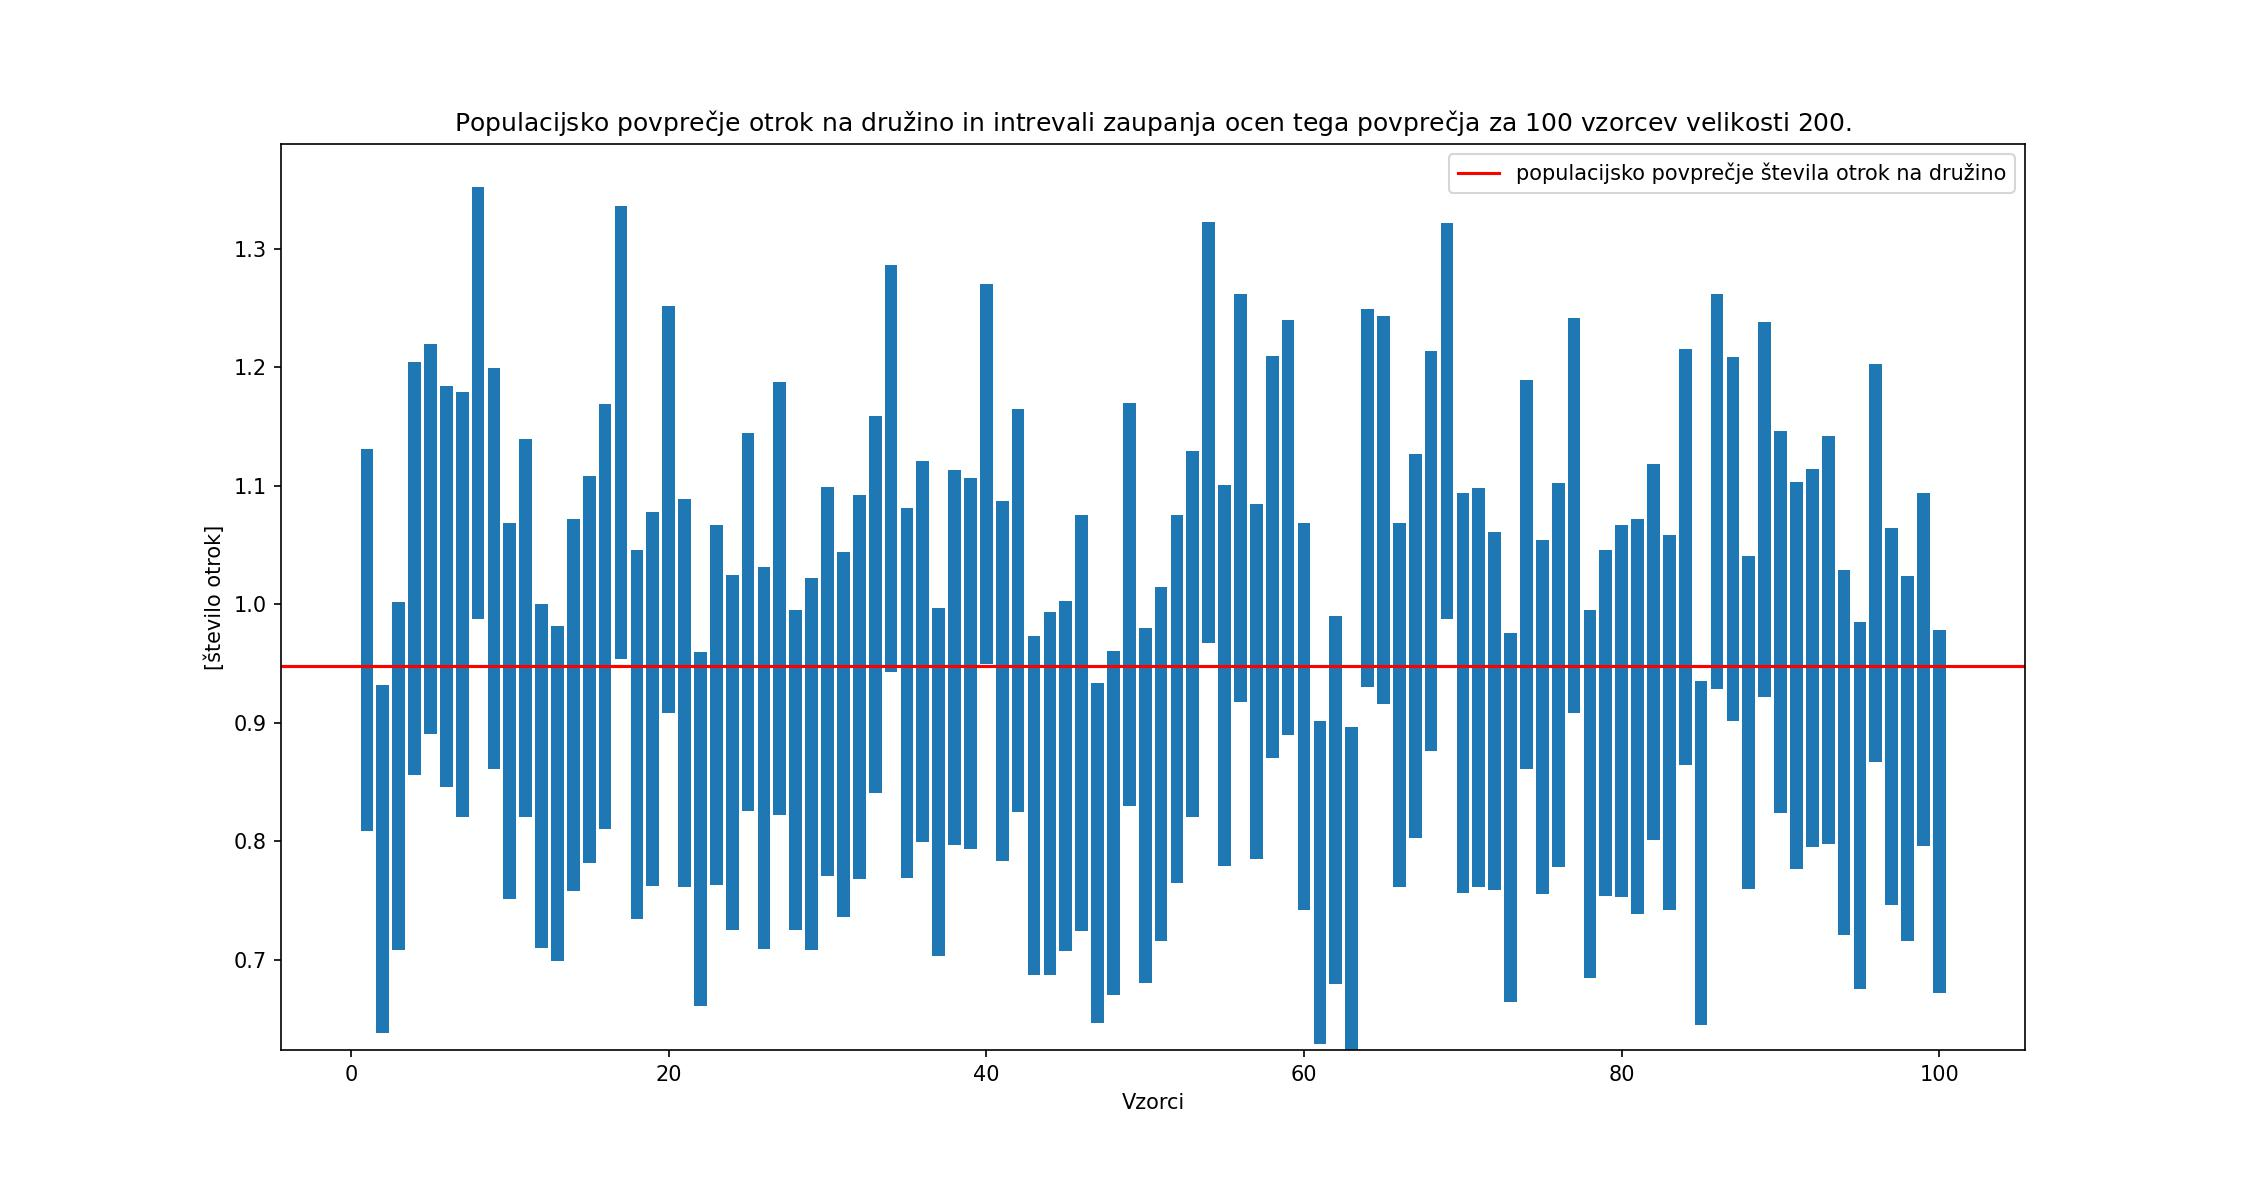
\includegraphics[scale=0.4]{../rezultati/intervali_zaupanja_100_vzorcev_pop_povprecje.jpg}
\end{figure}

Izračunamo, da populacijsko povprečje pokrije $96$ intervalov zaupanja, oz. delež intervalov, ki pokrijejo populacijsko povprečje, je $0{,}96$.

\subsection*{(e)}
Če označimo $i$-to oceno povprečja iz $i$-tega vzorca z $\mu_i$ in z $\overline{\mu}$ označimo povprečje teh ocen, je potem ocena za varianco teh ocen enaka
\begin{equation*}
    \widehat{\sigma}^2 =  \frac{1}{100 - 1} \sum_{i=1}^{100} (\mu_i - \overline{\mu})^2.
\end{equation*}
Torej je standardni odklon enak
\begin{equation*}
    \widehat{\sigma} = 0{,}0776.
\end{equation*}
Prava standardna napaka za vzorec velikosti $200$ pa je
\begin{equation*}
    \std_err = 0{,}0816,
\end{equation*}
kar vemo že od prej. Opazimo, da je standardni odklon ocen povprečja manjši od standardne napake.

\subsection*{(f)}
Tedaj so rezultati o intervalih zaupanja shranjeni v datoteki \texttt{intervali\char`_zaupanja\char`_1.csv} v mapi \texttt{rezultati}. Grafično je v tem primeru
\begin{figure}[H]
    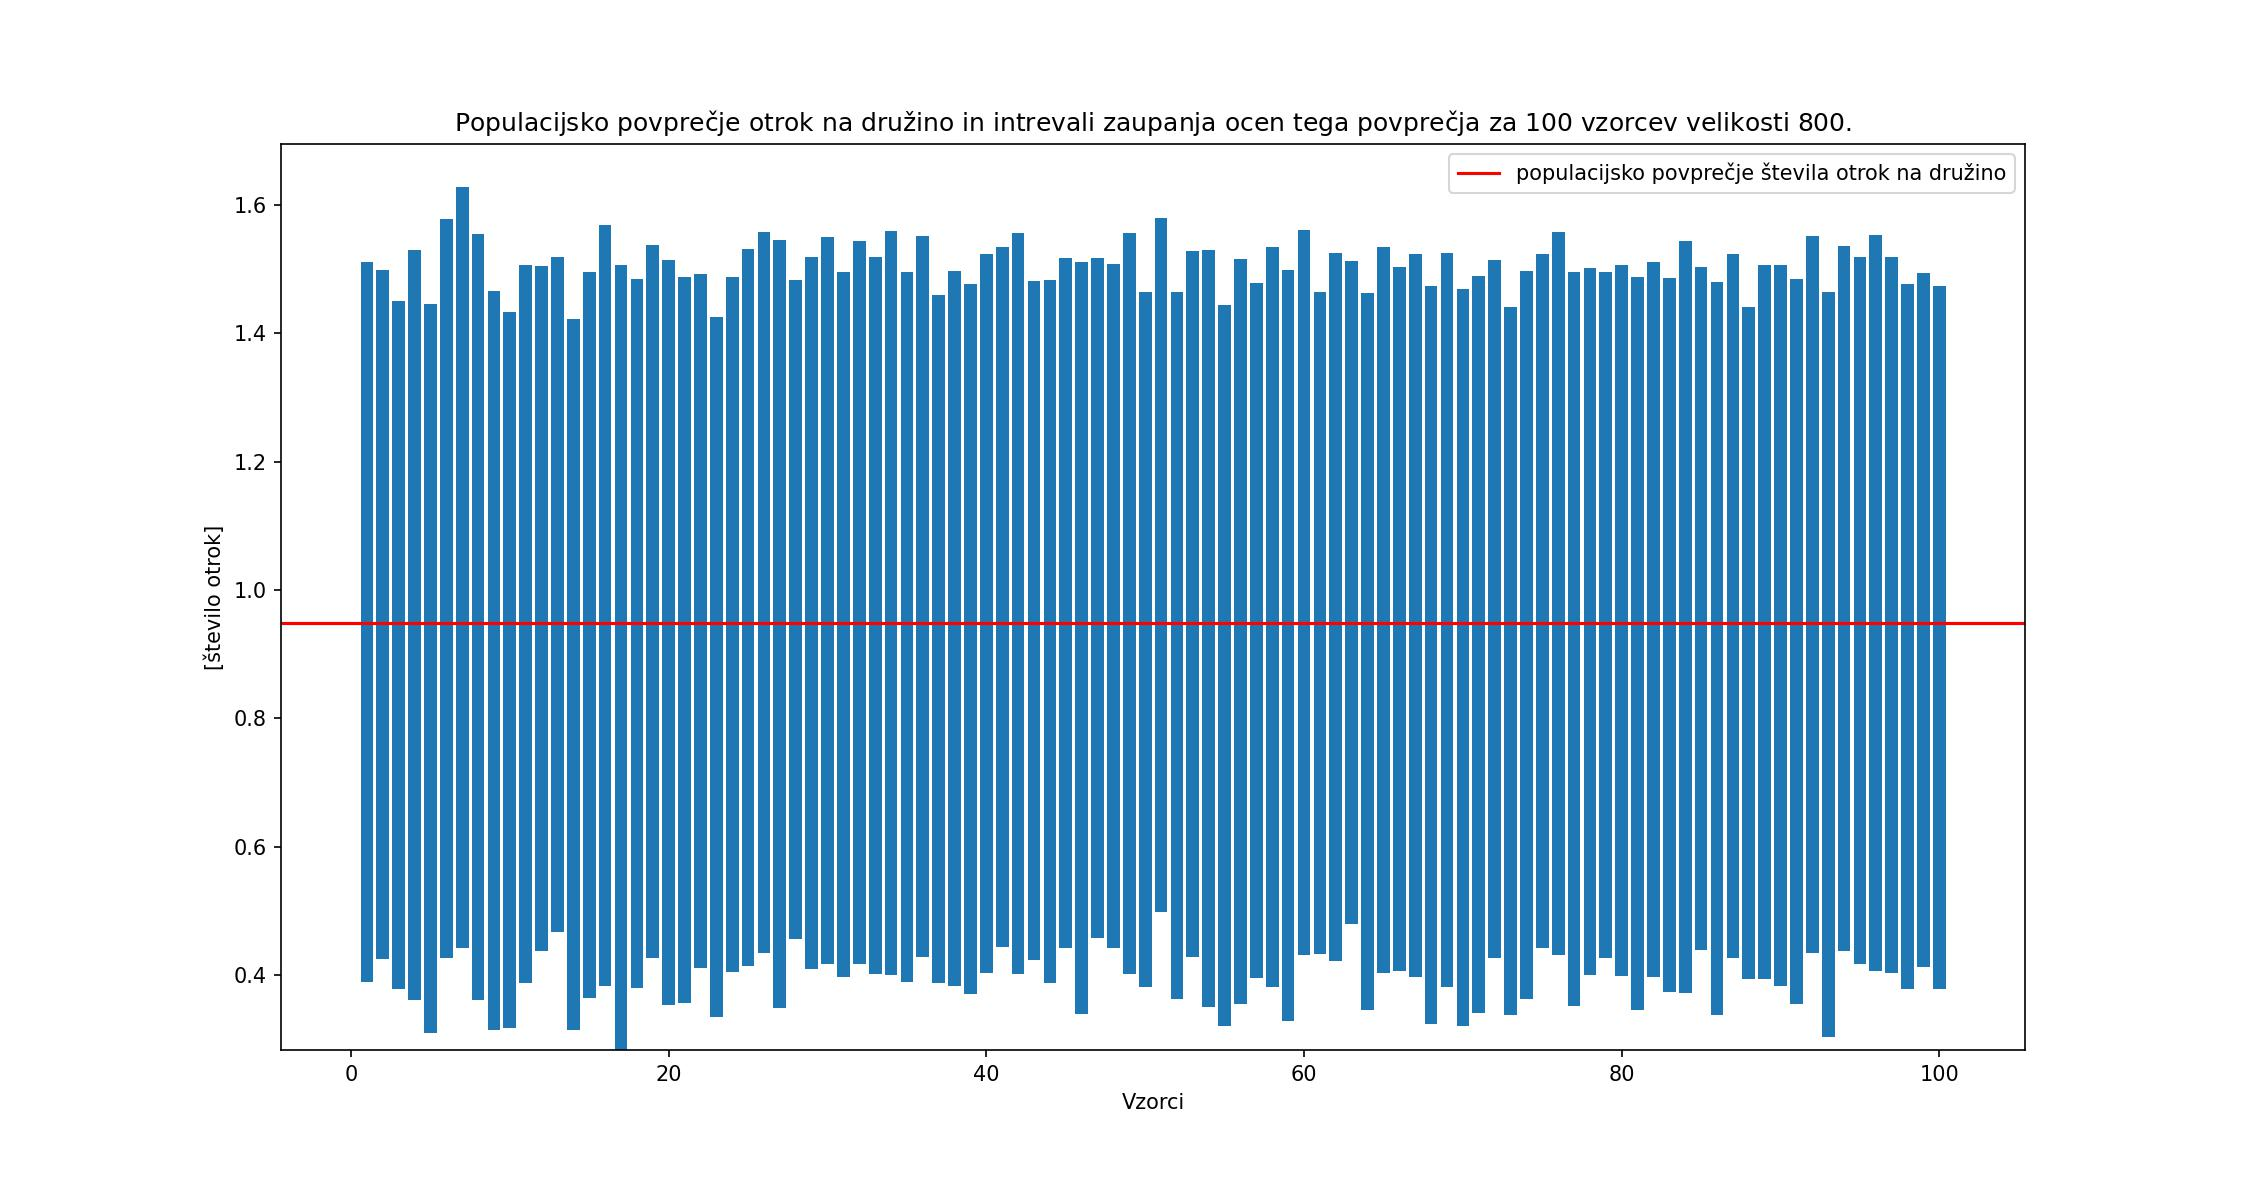
\includegraphics[scale=0.4]{../rezultati/intervali_zaupanja_100_vecjiih_vzorcev_pop_povprecje.jpg}
\end{figure}
Takoj opazimo, oziroma preverimo računsko, da tedaj intervali zaupanja vsi pokrijejo populacijsko povprečje. 

V tem primeru je standardni odklon ocen za povprečje enak
\begin{equation*}
    \widehat{\sigma}_1 = 0{,}0399.
\end{equation*}
Prava standardna napaka za vzorec velikosti $800$ pa je
\begin{equation*}
    \std_err_1 = 0{,}0405.
\end{equation*}

\end{document}